%% jan. 4, 2011  items to fix:
%% notation for math and reference to images.
%% how include eps figures.
%% make all the little figures (search for eps) in a common, nice matlab way for the
%% example filtering operations.

\chapter{Spatial filters}

The Fourier Transform is an indispensable tool for linear systems analysis,
image analysis, and for efficient filter output computation.
Among the benefits of the Fourier transform representation:  it's easy
to analyze images according to spatial frequency, and this represents some
progress in interpreting the image over merely a
pixel representation.  But the Fourier transform has a major drawback
as an image representation: it's too global!  Every sinusoidal
component covers the entire image.  The Fourier transform tells us a
little about {\em what} is happening in the image (based on the spatial
frequency content), but it tells us nothing about {\em where} it is happening.

On the other hand, a pixel representation gives great spatial localization, but a pixel
value by itself doesn't help us learn much about what's going on in
the image.  A Fourier representation tells us a bit about what's going
on, but nothing about where it happens.  We seek a representation
that's somewhere in between those two extremes.



In this chapter we will analyze several important linear filters. We will study spatial filters and then temporal filters.



\section{Human visual system and the contrast sensitivity function}

\begin{figure}
	\centerline{
		\includegraphics[width=1\linewidth]{figures/spatial_filters/csf.png}
	}
	\caption{Contrast sensitivity function shown by the Campbell \& Robson chart.}
	\label{fig:csfchart}
\end{figure}


Before we start describing different types of linear filters, let's start by gaining some subjective experience by playing with one: our own visual system. Although our visual system is clearly a non-linear system, linear filter theory can explain some aspects of our perception. Indeed, under certain conditions, the first stages of visual computation perform of the visual system can be approximated by a linear filter.

To experience the transfer function of our own visual system, let's build the following $N \times M$ image:
\begin{equation}
	\img \left[n,m\right] = A\left[m\right] \sin(2 \pi f\left[n\right] n/N)
\end{equation}
with
\begin{equation}
	A\left[m\right] = A_{min} \left(\frac{A_{max}}{A_{min}}\right)^{m/M}
\end{equation}
and
\begin{equation}
	f\left[n\right] = f_{min} \left(\frac{f_{max}}{f_{min}}\right)^{n/N}
\end{equation}
This image is separable and it is composed of two factors: an amplitude, $A\left[m\right]$, that varies only along the vertical dimension, and a wave with a frequency, $f\left[n\right]$, that varies along the horizontal component. We set the amplitude so that it is $A_{max}$ in the lowest part of the image and it decreases logarithmically to $A_{min}$ at the top. And the frequency function is defined as an increasing function that starts from 0 and grows up to 60 (with $N=2048$ being the number of horizontal pixels in the image). This image is shown in figure~\ref{fig:csfchart} and it is also called the Campbell \& Robson chart. It shows a signal with a wave that oscillates slow at the left and faster towards the right and that has high contrast a the bottom and loses contrast towards the top becoming invisible.

The first sign that our visual system is non-linear is that we do not perceive the amplitude as changing logarithmically from top to bottom. It feels more linear. This is because our photo-receptors compute the $\log$ of the incoming intensity (approximately).

What is interesting is that figure~\ref{fig:csfchart} is not perceived as being separable. If you trace the region where the sine wave seems to disappears you will trace a curve. In fact, your visual system is behaving as a band-pass filter: you are sensitive to middle spatial frequencies (with a pick around 6 cycles/degree) and you are less sensitive for very low spatial frequencies (left of the image) and to high-spatial frequencies (right of the image). This curve is called the contrast sensitivity function (CSF) in the psychophysics literature and is closely related to the transfer function of the filter.

The CSF is not a simple linear function but it can be approximated by one under certain conditions. However, the CSF changes depending of many factors such as overall intensity (the pick moves towards the left under low illumination. ), adaptation (long exposure to one frequency reduces the sensitivity for that frequency), age, ...

The DFT and use of sine waves became very popular in the study of visual psychophysics.

%
%
%Michelson contrast:
%\begin{equation}
%(Imax-Imin)/(Imax+Imin)  
%\end{equation}
%
%Weber contrast:  $\Delta I / I$.
%


\section{Low-pass filters}

%We will start by studying several important linear spatially invariant filters. These filters can be implemented as convolutions between an input image and a linear kernel.

\subsection{Box filter}

Let's start with a very simple filter, the box filter.  In the box filter, each output pixel is the sum of the input pixels around its neighborhood. The box convolution kernel can be written as:
\begin{equation}
	h_{N,M} \left[n,m \right] =
	\begin{cases}
		1 & \quad \text{if } -N \leq n \leq N  \text{~and~}  -M \leq m \leq M \\
		0 & \quad \text{otherwise }
	\end{cases}
\end{equation}
The box filter is separable as it can be written as the convolution of two 1D kernels: $h_{N,M} \left[n,m \right]  = h_{N,0} \circ h_{0,M}$.

Filtering an image with the box filter results in blurring the picture. Figure~\ref{fig:convExamps2} shows some box filters and the corresponding output images. Figure~\ref{fig:convExamps2}~(a) shows an image convolved with a uniform, rectangular kernel. Each pixel is an average of the input pixels within the rectangle. Figure~\ref{fig:convExamps2}~(b) and (c)  show the results of blurring in just one direction. Blur happens very often in real life. It happens when we look at something very far away, or at some detail inside a picture, or when we remove our eyeglasses (or wear some that are not ours).

\begin{figure}
	$
		\begin{array}{ccc}
			\text{a)}
			\includegraphics[width=.3\linewidth]{figures/spatial_filters/img1.jpg}
			 &
			\text{b)}
			\includegraphics[width=.15\linewidth]{figures/spatial_filters/street_square_kernel.jpg}
			 &
			\text{c)}
			\includegraphics[width=.3\linewidth]{figures/spatial_filters/street_square.jpg}
			\\
			\text{d)}
			\includegraphics[width=.3\linewidth]{figures/spatial_filters/img1.jpg}
			 &
			\text{e)}
			\includegraphics[width=.15\linewidth]{figures/spatial_filters/street_horizontal_kernel.jpg}
			 &
			\text{f)}
			\includegraphics[width=.3\linewidth]{figures/spatial_filters/street_horizontal.jpg}
			\\
			\text{g)}
			\includegraphics[width=.3\linewidth]{figures/spatial_filters/img1.jpg}
			 &
			\text{h)}
			\includegraphics[width=.15\linewidth]{figures/spatial_filters/street_vertical_kernel.jpg}
			 &
			\text{i)}
			\includegraphics[width=.3\linewidth]{figures/spatial_filters/street_vertical.jpg}
		\end{array}
	$
	%\centerline{
	%\sublabel{a}{
	%\includegraphics[width=0.75\linewidth]{figures/intro_signals/conv4.pdf}}}
	%\centerline{
	%\sublabel{b}{
	%\includegraphics[width=0.75\linewidth]{figures/intro_signals/conv5.pdf}}}
	%\centerline{
	%\sublabel{c}{
	%\includegraphics[width=0.75\linewidth]{figures/intro_signals/conv6.pdf}}}
	\caption{Blurring with (a) a rectangle, and  a (b) horizontal and (c)
		vertical line.  Note the structures that are both averaged out
		(along the direction of blurring), and
		maintained (perpendicular to that direction) in each resulting image.
	}
	\label{fig:convExamps2}
\end{figure}



The box filter is simple but it has a number of issues:
\begin{itemize}
	\item {If you convolve two boxes you get a triangle. You can easily check this. For instance, in the simple case where $N=1, M=0$:
	      \begin{equation}
		      h_{1,0}  \circ h_{1,0} = \left[1, 1, 1\right] \circ \left[1, 1, 1\right] = \left[1,2,3,2,1\right]
	      \end{equation}
	      the output  is a triangular filter with length $2\times L-1$, with $L=3$ the length of the box filter. Although that is not a problem at first sight, it means that if you blur an image twice with box filters, what you get is not equivalent to blurring only once with a larger box filter. }

	\item {The box filter is not a perfect blurring filter. A blur filter should attenuate high spatial frequencies with stronger attenuation for higher spatial frequencies. However, if you consider the highest spatial frequency, which will be an oscillating signal that takes successively on the values 1 and -1: $\left[..., 1, -1, 1, -1, 1, -1, ... \right]$ when filtered with the box filter $h_{1,0}$ the results is the same signal! However, if you filter a wave with lower frequency such as $\left[..., 0.5, 0.5, -1, 0.5, 0.5, -1, ... \right]$ then the result is $\left[..., 0,0,0,0, ...\right]$. Therefore, the attenuation is not monotonic with spatial frequency as it is shown in figure \ref{fig:boxfilter}. This is not a desirable behavior for a blurring filter and it can cause artifacts to appear. This could be addressed using an even size box filter $\left[1,1 \right]$. However, an even box filter is not centered around the origin and the output image will have a half-pixel translation. Therefore, odd filter sizes are preferred.}
\end{itemize}


\begin{figure}[h]
	\begin{center}
		\[
			\begin{array}{cc}
				\text{a)}
				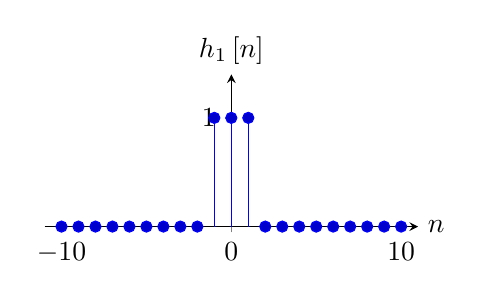
\begin{tikzpicture}
					\begin{axis} [width=180pt,height=100pt,
							axis x line=bottom,
							axis y line=middle,
							tick align=center,
							every axis x label/.style={at={(current axis.right of origin)},anchor=west},
							every axis y label/.style={at={(current axis.above origin)}, anchor=north east,above=0mm},
							xmin=-11, xmax=11,
							xtick={-10, 0, 10},
							xlabel=$n$,
							ymin=0, ymax=1.4,
							ytick={0,...,1},
							ylabel={$h_1 \left[n\right]$}]
						\addplot+[ycomb] plot coordinates {(-10,0) (-9,0) (-8,0) (-7,0) (-6,0) (-5,0) (-4,0) (-3,0) (-2,0) (-1,1) (0,1) (1,1) (2,0) (3,0) (4,0) (5,0) (6,0) (7,0) (8,0) (9,0) (10,0)};
					\end{axis}
				\end{tikzpicture}

				\text{b)}
				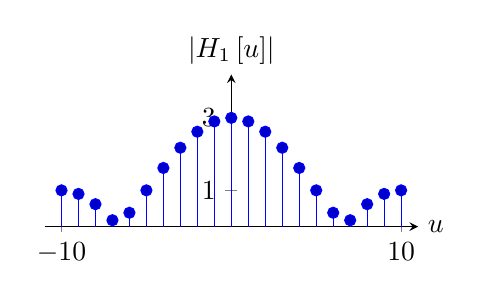
\begin{tikzpicture}
					\begin{axis} [width=180pt,height=100pt,
							axis x line=middle,
							axis y line=middle,
							tick align=center,
							every axis x label/.style={at={(current axis.right of origin)},anchor=west},
							every axis y label/.style={at={(current axis.above origin)}, anchor=north east,above=0mm},
							xmin=-11, xmax=11,
							xtick={-10, 0,10},
							xlabel=$u$,
							ymin=0, ymax=4.2,
							ytick={0,1,3},
							ylabel={$\left| H_1 \left[ u \right] \right|$},
							color=black]
						\addplot+[ycomb,domain=-10:10,samples=21,samples y=0]
						({x}, {abs(1+2*cos(deg(2*pi*x*1/20)))});
					\end{axis}
				\end{tikzpicture}
			\end{array}
		\]
	\end{center}
	\caption{a) A one dimensional box filter ($\left[1,1,1\right]$) and b) its Fourier transform over 20 samples. Note that the frequency gain is not monotonically decreasing with spatial frequency.}
	\label{fig:boxfilter}
\end{figure}


The next blurring filter addresses both of these issues.

\subsection{Gaussian filter}
\label{sec:spt_gaussian}

One of the important blurring (low-pass) filters in computer vision is the gaussian filter. The gaussian filter is important because it is a good model for many naturally occurring filters. It also has a number of properties, as we will discuss here, that make it unique.

The gaussian distribution is defined in continuous variables. In one dimension:
\begin{equation}
	g(x; \sigma) = \frac{1}{\sqrt{2 \pi \sigma^2}} \exp{-\frac{x^2}{2 \sigma^2}}
	\label{eq:gauss1dcont}
\end{equation}
and in 2 dimensions:
\begin{equation}
	g(x,y; \sigma) = \frac{1}{2 \pi \sigma^2} \exp{-\frac{x^2 +
			y^2}{2 \sigma^2}}
	\label{eq:gauss2dcont}
\end{equation}
The parameter $\sigma$ adjusts the spatial extend of the gaussian. The normalization constant is set so that the function integrates to 1.

In order to use this filter in practice we need to consider discrete locations and also approximate the function by a finite support function. In practice, we only need to consider samples within three standard deviations $x \in (-3\sigma, 3\sigma)$. At $3\sigma$ the amplitude of the gaussian is around $1\%$ of its central value. Unfortunately, many of the properties of the gaussian that we will discuss later are only true in the continuous domain and are only approximated when using its discrete form.

For a given standard deviation parameter, $\sigma$, the discretized gaussian kernel is $g \left[m, n; \sigma \right]$:
\begin{equation}
	g \left[ m,n; \sigma \right] = \exp{-\frac{m^2 +
			n^2}{2 \sigma^2}}
	\label{eq:gauss2d}
\end{equation}
We have removed the normalization constant as the sum of the discrete gaussian will be different from the integral of the continuous function. So here we prefer to use the form in which the value at the origin is 1. In practice, we should normalize the discrete gaussian by the sum of its values to make sure that the gain at DC is 1.

By adjusting the standard deviation, $\sigma$, of the Gaussian, it is possible to adjust the level of image detail
that appears in the blurred image. Figure~\ref{fig:zebragaussian} shows the result of narrow and wider Gaussians applied to an image.


\begin{figure}
	$
		\begin{array}{ccc}
			\text{a)}
			\includegraphics[width=.3\linewidth]{figures/spatial_filters/gausian_zebra_c_2.jpg}
			 &
			\text{b)}
			\includegraphics[width=.3\linewidth]{figures/spatial_filters/gausian_zebra_c_4.jpg}
			 &
			\text{c)}
			\includegraphics[width=.3\linewidth]{figures/spatial_filters/gausian_zebra_c_8.jpg}
			\\
			\text{d)}
			\includegraphics[width=.3\linewidth]{figures/spatial_filters/gausian_c_2plot.jpg}
			 &
			\text{e)}
			\includegraphics[width=.3\linewidth]{figures/spatial_filters/gausian_c_4plot.jpg}
			 &
			\text{f)}
			\includegraphics[width=.3\linewidth]{figures/spatial_filters/gausian_c_8plot.jpg}
		\end{array}
	$
	\caption{An image filtered with three gaussians with standard deviations: a) $\sigma=2$, b) $\sigma=4$, and c) $\sigma=8$. Plots (d) - (f) show the three Gaussians over the same spatial support as the image. The discrete Gaussians are approximated by sampling the continuous Gaussian. The convolutions are perform with mirror boundary conditions. }
	\label{fig:zebragaussian}
\end{figure}





The multi-dimensional Gaussian filter has the additional computational advantage that it can
be applied as a concatenation of 1-d Gaussian filters.  This can be
seen by writing the 2-d Gaussian, Eq.~(\ref{eq:gauss2d}), in the
convolution equation, Eq.~(\ref{eq:linconv}).  Letting $g^x$
and $g^y$ be the 1-d Gaussian convolution kernels in the horizontal
and vertical directions, we have
\begin{eqnarray*}
	g \left[m,n \right] \circ f \left[m,n\right]
	& = & \sum_{k,l}
	g \left[m-k,n-l \right] f\left[k,l \right] \\
	& = & \sum_{k,l}
	%\frac{1}{2 \pi \sigma^2} 
	\exp{-\frac{(m-k)^2 + (n-l)^2}{2 \sigma^2}}
	\circ f \left[m,n \right] \\
	& = &
	\sum_{k}
	%\frac{1}{\sqrt{2 \pi \sigma^2}} 
	\exp{-\frac{(m-k)^2}{2 \sigma^2}}
	\left(
	\sum_{l}
	%\frac{1}{\sqrt{2 \pi \sigma^2}} 
	\exp{-\frac{(n-l)^2}{2 \sigma^2}} f \left[k,l \right]
	\right)
	\\
	& = &
	g^x \circ (g^y \circ f \left[m,n \right])
	\label{eq:2dgauss}
\end{eqnarray*}
This can save quite a bit in computation time when applying the
convolution of Eq.~(\ref{eq:2dgauss}).  If the 2-d convolution kernel
is $nxn$ samples, then a direct convolution of that 2-d kernel scales
in proportion to $n^2$, since Eq.~(\ref{eq:2dgauss}) requires one
multiplication per image position per kernel sample.  Using the
cascade of two 1-d kernels, resulting in an equivalent 2-d filter of
the same size, scales in proportion to $2n$.

Another application of blurring is to remove distracting
high-resolution image details.
Fig.~\ref{fig:lincoln} shows a Gaussian low-pass filter applied to
remove unwanted image details (the blocky artifacts) from an image.


Properties of the Gaussian filter:
\begin{itemize}
	\item The n-dimensional Gaussian is the only completely circularly symmetric operator that is separable.

	\item The continuous Fourier transform of a gaussian is also a gaussian.
	      \begin{equation}
		      G (u,v; \sigma) = \exp{- 2 \pi^2 (u^2 +  v^2) \sigma^2}
		      \label{eq:FTgauss2d}
	      \end{equation}
	      Note that this function is monotonically decreasing in magnitude for increasing frequencies, and it is also radially symmetric.

	\item The convolution of two n-dimensional gaussians is an n-dimensional gaussian.
	      \begin{equation}
		      g (x,y; \sigma_1 ) \circ g (x,y; \sigma_2)  = g (x,y; \sigma_3)
	      \end{equation}
	      where the variance of the result is the sum $\sigma_3^2 = \sigma_1^2 + \sigma_2^2$. This is a remarkable property of gaussian filters and is the basis of the gaussian pyramid that we will see later. To prove this property, one can use the Fourier transform of the gaussian and the fact that the convolution is the product of Fourier transforms.

	\item The gaussian is the solution to the heat equation.

	\item Repeated convolutions of any function concentrated in the origin result in a gaussian (central limit theorem).

	\item In the limit $\sigma \rightarrow 0$ the Gaussian becomes an impulse. This property is shared by many other functions, but it is a useful thing to know.
\end{itemize}

However, many of these properties do not work for the discrete approximation $g\left[n,m;\sigma \right]$ obtained by directly sampling the values of the gaussian at discrete locations. To see this let's look at some examples. Let's consider a gaussian with variance $\sigma^2=1/2$. It can be approximated by 5 samples. We will call this approximation $g_5$:
\begin{equation}
	g_5\left[ n \right] = \left[0.0183, \,    0.3679, \,    1.0000, \,    0.3679, \,    0.0183 \right]
\end{equation}
first, note when convolved with a wave $\left[1,-1,1,-1,...\right]$ the result is not zero. This is to be expected from the form of the FT of the gaussian. You can check that if you  compute the approximation for $\sigma^2=1$ by discretizing the gaussian, the result obtained is not equal to doing $g_5 \circ g_5$. Therefore, as you apply successive convolutions of gaussian the errors will accumulate.

\subsection{Binomial filters}

In practice, there are very efficient approximations to the Gaussian filter for certain $\sigma$ values with nicer properties than when working with discretized gaussians. One common approximation of the gaussian filter is to use binomial coefficients \cite{canny,Chehikian}. Binomial coefficients provide a compact approximation of the gaussian coefficients using only integers. The binomial coefficients use the central limit theorem to approximate a gaussian as successive convolutions of a very simple function. The simplest low-pass filter is the box filter $\left[1,1\right]$. The binomial coefficients form the Pascal's triangle as shown in figure \ref{fig:pascaltriangle}.

\begin{figure}[h]
	\centerline{
		%\[
		$\begin{array}{ccccccccccccccccccccccccl}
				b_0 & ~ & ~ & ~ & ~ & ~ & ~ & ~ & ~  & ~  & ~  & ~  & 1  & ~  & ~  & ~  & ~  & ~ & ~ & ~ & ~ & ~ & ~ & ~ & \sigma_0^2=0   \\
				b_1 & ~ & ~ & ~ & ~ & ~ & ~ & ~ & ~  & ~  & ~  & 1  & ~  & 1  & ~  & ~  & ~  & ~ & ~ & ~ & ~ & ~ & ~ & ~ & \sigma_1^2=1/4 \\
				b_2 & ~ & ~ & ~ & ~ & ~ & ~ & ~ & ~  & ~  & 1  & ~  & 2  & ~  & 1  & ~  & ~  & ~ & ~ & ~ & ~ & ~ & ~ & ~ & \sigma_2^2=1/2 \\
				b_3 & ~ & ~ & ~ & ~ & ~ & ~ & ~ & ~  & 1  & ~  & 3  & ~  & 3  & ~  & 1  & ~  & ~ & ~ & ~ & ~ & ~ & ~ & ~ & \sigma_3^2=3/4 \\
				b_4 & ~ & ~ & ~ & ~ & ~ & ~ & ~ & 1  & ~  & 4  & ~  & 6  & ~  & 4  & ~  & 1  & ~ & ~ & ~ & ~ & ~ & ~ & ~ & \sigma_4^2=1   \\
				b_5 & ~ & ~ & ~ & ~ & ~ & ~ & 1 & ~  & 5  & ~  & 10 & ~  & 10 & ~  & 5  & ~  & 1 & ~ & ~ & ~ & ~ & ~ & ~ & \sigma_5^2=5/4 \\
				b_6 & ~ & ~ & ~ & ~ & ~ & 1 & ~ & 6  & ~  & 15 & ~  & 20 & ~  & 15 & ~  & 6  & ~ & 1 & ~ & ~ & ~ & ~ & ~ & \sigma_6^2=3/2 \\
				b_7 & ~ & ~ & ~ & ~ & 1 & ~ & 7 & ~  & 21 & ~  & 35 & ~  & 35 & ~  & 21 & ~  & 7 & ~ & 1 & ~ & ~ & ~ & ~ & \sigma_7^2=7/4 \\
				b_8 & ~ & ~ & ~ & 1 & ~ & 8 & ~ & 28 & ~  & 56 & ~  & 70 & ~  & 56 & ~  & 28 & ~ & 8 & ~ & 1 & ~ & ~ & ~ & \sigma_8^2=2
			\end{array}$
		%\]
	}
	\caption{Binomial coefficients. To build the Pascal's triangle, each number is the sum of the number above to the left and the one above to the right.}
	\label{fig:pascaltriangle}
\end{figure}

The sum of all the coefficients for each binomial filter $b_n$ is $2^n$, and their variance is $\sigma^2 = n/4$. One remarkable property of the binomial filters is that $b_n \circ b_m = b_{n+m}$, and, therefore, $\sigma_n^2 + \sigma_m^2  = \sigma_{n+m}^2$, which is the analogous to the gaussian property in the continuous domain. Note that the values of $b_2$ are different from $g_5$ despite that both will be used as approximations to the same gaussian.

The simplest approximation to the Gaussian filter is the 3-tap kernel:
\begin{equation}
	b_2 = \left[1, 2, 1\right]
\end{equation}
This filter is interesting because it is even (so it can be applied to an image without producing any translation) and its DFT is:
\begin{equation}
	B_2 \left[u\right] = 2+2 \cos (2 \pi u/N)
\end{equation}
it has a monotonic amplitude gain in frequency (there are no ripples) as shown in figure \ref{fig:gauss3filter}.  All the even binomial filters can be written as successive convolutions with the kernel $\left[1,2,1\right]$. Therefore, their Fourier transform is a power of the Fourier transform of the filter $\left[1,2,1\right]$ and therefore they are also monotonic:
\begin{equation}
	B_{2n} \left[u\right] = (2+2 \cos (2 \pi u/N))^n
\end{equation}
For all the binomial filters $b_n$, when they are convolved with the wave $\left[1,-1,1,-1,...\right]$, the result is the zero signal $\left[0,0,0,0,...\right]$. This is a very nice property of binomial filters and will become very useful later when talking about downsampling an image (see section \ref{}).

\begin{figure}[h]
	\begin{center}
		\[
			\begin{array}{cc}
				\text{a)}
				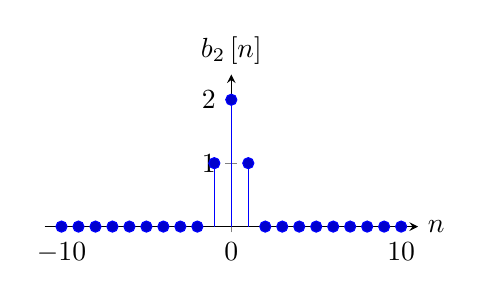
\begin{tikzpicture}
					\begin{axis} [width=180pt,height=100pt,
							axis x line=bottom,
							axis y line=middle,
							tick align=center,
							every axis x label/.style={at={(current axis.right of origin)},anchor=west},
							every axis y label/.style={at={(current axis.above origin)}, anchor=north east,above=0mm},
							xmin=-11, xmax=11,
							xtick={-10, 0, 10},
							xlabel=$n$,
							ymin=0, ymax=2.4,
							ytick={0,...,2},
							ylabel={$b_2 \left[n\right]$}]
						\addplot+[ycomb] plot coordinates {(-10,0) (-9,0) (-8,0) (-7,0) (-6,0) (-5,0) (-4,0) (-3,0) (-2,0) (-1,1) (0,2) (1,1) (2,0) (3,0) (4,0) (5,0) (6,0) (7,0) (8,0) (9,0) (10,0)};
					\end{axis}
				\end{tikzpicture}

				\text{b)}
				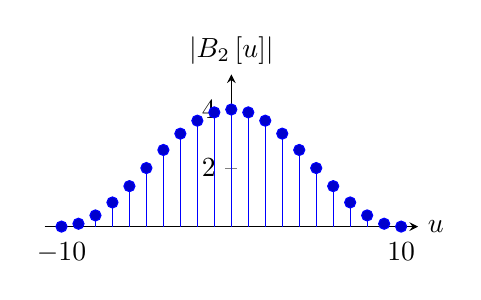
\begin{tikzpicture}
					\begin{axis} [width=180pt,height=100pt,
							axis x line=middle,
							axis y line=middle,
							tick align=center,
							every axis x label/.style={at={(current axis.right of origin)},anchor=west},
							every axis y label/.style={at={(current axis.above origin)}, anchor=north east,above=0mm},
							xmin=-11, xmax=11,
							xtick={-10, 0,10},
							xlabel=$u$,
							ymin=0, ymax=5.2,
							ytick={0,2,4},
							ylabel={$\left| B_2 \left[ u \right] \right|$},
							color=black]
						\addplot+[ycomb,domain=-10:10,samples=21,samples y=0]
						({x}, {abs(2+2*cos(deg(2*pi*x*1/20)))});
					\end{axis}
				\end{tikzpicture}
			\end{array}
		\]
	\end{center}
	\caption{a) A one dimensional 3-tap approximation to the gaussian filter ($\left[1,2,1\right]$) and b) its Fourier transform over 20 samples. Note that the frequency gain is decreasing monotonically with spatial frequency and it becomes zero at the highest frequency, $G_3 \left[ 10 \right]=0$.}
	\label{fig:gauss3filter}
\end{figure}

The gaussian in 2D can be approximated, using separability, as the convolution of two binomial filters one vertical and another horizontal. For instance:
\begin{equation}
	b_{2,2} = b_{2,0} \circ b_{0,2} =  \begin{bmatrix}
		1 ~ & 2 ~ & 1 \\
	\end{bmatrix}\circ \begin{bmatrix}
		1 \\
		2 \\
		1
	\end{bmatrix}=
	% =
	% 
	\begin{bmatrix}
		1 ~ & 2 ~ & 1 \\
		2 ~ & 4 ~ & 2 \\
		1~  & 2 ~ & 1
	\end{bmatrix}
\end{equation}


\begin{figure}
	\centerline{
		\includegraphics[width=0.55\linewidth]{figures/spatial_filters/lincoln.pdf}}
	\caption{Left:  input image.  Right:  blurred version.  The left
		version has many spurious details introduced by the undersampling of
		the image.  The right image has been blurred by a large Gaussian
		filter.  ((image from
		http://acor.org/sgreene/hmsbeagle/html/content/17/recroom/artgalas.htm,
		after 1973 image by Bela Julesz and Leon Harmon )).
	}
	\label{fig:lincoln}
\end{figure}


What is the inverse? can we remove gaussian filter? Show the matrix for some simple case and show it does not behave nicely.

Due to all these properties the gaussian and the binomial filter are extensively used in computer vision.


\section{High-pass filters}


\subsection{Image derivatives}

Computing image derivatives is an essential operator for extracting useful information from images. As we show in the previous chapter, image derivatives allowed us computing boundaries between objects and to have access to some of the 3D information lost when projecting the 3D world into the camera plane.  Derivatives are useful because they give us information about where are happening the changes in the image and we expect those changes to be correlated with transitions between objects.


If we had access to the continuous image, then image derivatives could be computed as: $\partial \img(x,y) / \partial x$. However, there are two reasons why we might not be able to apply this definition
\begin{itemize}
	\item the first one is that we only have access to a sampled version of the input image: $\img \left[m,n\right]$
	\item even if we had access to the continuous image, the image could contain many non-derivable points and the gradient would not be defined. We will see how to address this issue later when we study gaussian derivatives.
\end{itemize}
for now, let's focus on the problem of approximating the continuous derivative with discrete operators. As the derivative is a linear operator, it can be approximated by a discrete linear filter. There are several ways in which image derivatives can be approximated.

Let's start with a simple approximation to the derivative operator that we have already played with: $d_0  = \left[1, -1 \right]$. In one dimension, convolving a signal $f \left[n \right]$ with this filter results in:
\begin{equation}
	f \circ d_0 = f \left[n \right] - f \left[n-1 \right]
\end{equation}
this approximates the derivative by the difference between consecutive values. Figure~\ref{fig:discretederivative}.c shows the result of filtering a 1-d signal (fig.\ref{fig:discretederivative}.a) convolved with $d_0 \left[n\right]$ (fig.\ref{fig:discretederivative}.b). The output is zero wherever the input signal is constant and it is large in the places where there are variations in the input values. However note that the output is not perfectly aligned with the input. In fact there is a half a sample displacement to the right. This is due to the fact that $d_0 \left[n\right]$ is not centered around the origin.

This can be addressed with a different approximation to the spatial derivative: $d_1  = \left[1, 0, -1 \right]/2$. In one dimension, convolving a signal $f \left[n \right]$ with $d_1 \left[n\right]$ results in:
\begin{equation}
	f \circ d_1 = \frac{f \left[n+1 \right] - f \left[n-1 \right]}{2}
\end{equation}
Figure~\ref{fig:discretederivative}.e shows the result of filtering the 1-d signal (fig.\ref{fig:discretederivative}.a) convolved with $d_1 \left[n\right]$ (fig.\ref{fig:discretederivative}.d). Now the output shows the highest magnitude output in the mid point where there is variation in the input signal.

\begin{figure}[h]
	\begin{center}
		$
			\begin{array}{lcr}
				~ & ~ &
				\text{a)}
				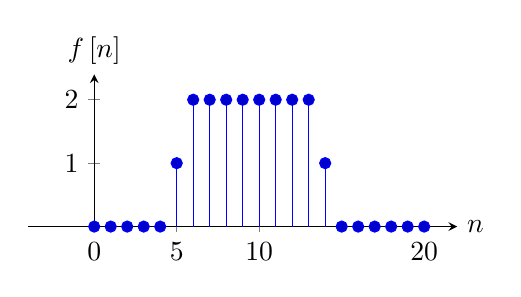
\begin{tikzpicture}
					\begin{axis} [width=200pt,height=100pt,
							axis x line=bottom,
							axis y line=middle,
							tick align=center,
							every axis x label/.style={at={(current axis.right of origin)},anchor=west},
							every axis y label/.style={at={(current axis.above origin)}, anchor=north east,above=0mm},
							xmin=-4, xmax=22,
							xtick={0, 5,10, 20},
							xlabel=$n$,
							ymin=0, ymax=2.4,
							ytick={0,...,2},
							ylabel={$f \left[n\right]$}]
						\addplot+[ycomb] plot coordinates {(0,0) (1,0) (2,0) (3,0) (4,0) (5,1) (6,2) (7,2) (8,2) (9,2) (10,2) (11,2) (12,2) (13,2) (14,1) (15,0) (16,0) (17,0) (18,0) (19,0) (20,0)};
					\end{axis}
				\end{tikzpicture}
				\\
				\text{b)}
				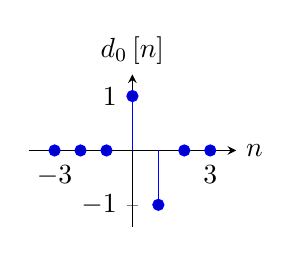
\begin{tikzpicture}
					\begin{axis} [width=120pt,height=100pt,
							axis x line=middle,
							axis y line=middle,
							tick align=center,
							every axis x label/.style={at={(current axis.right of origin)},anchor=west},
							every axis y label/.style={at={(current axis.above origin)}, anchor=north east,above=0mm},
							xmin=-4, xmax=4,
							xtick={-3,3},
							xlabel=$n$,
							ymin=-1.4, ymax=1.4,
							ytick={-1,0,1},
							ylabel={$d_0 \left[n\right]$},
							color=black]
						\addplot+[ycomb] plot coordinates {(-3,0) (-2,0) (-1,0) (0,1) (1,-1) (2,0) (3,0) };
					\end{axis}
				\end{tikzpicture}
				  &
				~
				  &
				\text{c)}
				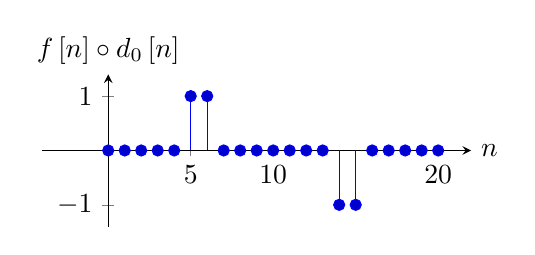
\begin{tikzpicture}
					\begin{axis} [width=200pt,height=100pt,
							axis x line=middle,
							axis y line=middle,
							tick align=center,
							every axis x label/.style={at={(current axis.right of origin)},anchor=west},
							every axis y label/.style={at={(current axis.above origin)}, anchor=north east,above=0mm},
							xmin=-4, xmax=22,
							xtick={0, 5, 10, 20},
							xlabel=$n$,
							ymin=-1.4, ymax=1.4,
							ytick={-1,...,1},
							ylabel={$f \left[n\right] \circ d_0 \left[n\right]$}]
						%\addplot+[ycomb] plot coordinates {(0,0) (1,0) (2,0) (3,0) (4,0) (5,1) (6,2) (7,2) (8,2) (9,2) (10,2) (11,2) (12,2) (13,2) (14,1) (15,0) (16,0) (17,0) (18,0) (19,0) (20,0)};
						\addplot+[ycomb] plot coordinates {(0,0) (1,0) (2,0) (3,0) (4,0) (5,1) (6,1) (7,0) (8,0) (9,0) (10,0) (11,0) (12,0) (13,0) (14,-1) (15,-1) (16,0) (17,0) (18,0) (19,0) (20,0)};
					\end{axis}
				\end{tikzpicture}
				\\
				\text{d)}
				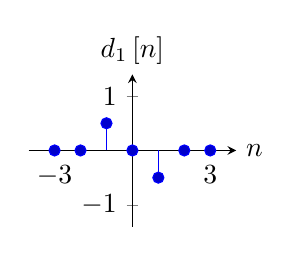
\begin{tikzpicture}
					\begin{axis} [width=120pt,height=100pt,
							axis x line=middle,
							axis y line=middle,
							tick align=center,
							every axis x label/.style={at={(current axis.right of origin)},anchor=west},
							every axis y label/.style={at={(current axis.above origin)}, anchor=north east,above=0mm},
							xmin=-4, xmax=4,
							xtick={-3,3},
							xlabel=$n$,
							ymin=-1.4, ymax=1.4,
							ytick={-1,0,1},
							ylabel={$d_1 \left[n\right]$},
							color=black]
						\addplot+[ycomb] plot coordinates {(-3,0) (-2,0) (-1,1/2) (0,0) (1,-1/2) (2,0) (3,0) };
					\end{axis}
				\end{tikzpicture}
				  &
				~
				  &
				\text{e)}
				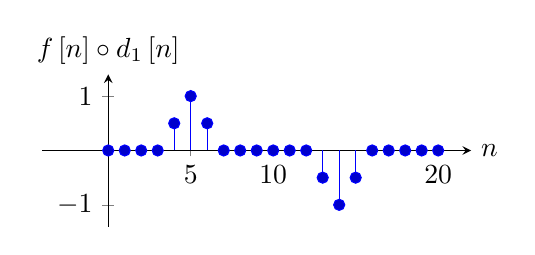
\begin{tikzpicture}
					\begin{axis} [width=200pt,height=100pt,
							axis x line=middle,
							axis y line=middle,
							tick align=center,
							every axis x label/.style={at={(current axis.right of origin)},anchor=west},
							every axis y label/.style={at={(current axis.above origin)}, anchor=north east,above=0mm},
							xmin=-4, xmax=22,
							xtick={0, 5,10, 20},
							xlabel=$n$,
							ymin=-1.4, ymax=1.4,
							ytick={-1,...,1},
							ylabel={$f \left[n\right] \circ d_1 \left[n\right]$}]
						%\addplot+[ycomb] plot coordinates {(0,0) (1,0) (2,0) (3,0) (4,0) (5,1) (6,2) (7,2) (8,2) (9,2) (10,2) (11,2) (12,2) (13,2) (14,1) (15,0) (16,0) (17,0) (18,0) (19,0) (20,0)};
						\addplot+[ycomb] plot coordinates {(0,0) (1,0) (2,0) (3,0) (4,1/2) (5,1) (6,1/2) (7,0) (8,0) (9,0) (10,0) (11,0) (12,0) (13,-1/2) (14,-1) (15,-1/2) (16,0) (17,0) (18,0) (19,0) (20,0)};
					\end{axis}
				\end{tikzpicture}
			\end{array}
		$
	\end{center}
	\caption{a) b).}
	\label{fig:discretederivative}
\end{figure}

It is also interesting to see the behavior of the derivative and its discrete approximations in the Fourier domain.

\begin{equation}
	d f(x) / dx  \leftrightarrow  j w F(w)
\end{equation}
in the continuous Fourier domain, derivation can be done by multiplying by $jw$.
The DFT of $d_0 \left[n\right]$ is:
\begin{equation}
	\begin{split}
		D_0 \left[u \right] = & 1 - \exp \left( -2 \pi j \frac{u}{N} \right) =                                                                                            \\
		                      & = \exp \left( - \pi j \frac{u}{N} \right) \left(  \exp \left( \pi j \frac{u}{N} \right) - \exp \left( -\pi j \frac{u}{N} \right)  \right) \\
		                      & = \exp \left( - \pi j \frac{u}{N} \right) 2 j \sin (\pi u /N)
	\end{split}
\end{equation}
the first term is a pure phase shift and it is responsible of the half a sample delay in the output. The second term is the amplitude gain and it can be approximated by a linear dependency on $u$ for small $u$ values.

The DFT of $d_1 \left[n\right]$ is:
\begin{equation}
	\begin{split}
		D_1 \left[u \right] = & 1/2\exp \left( 2 \pi j \frac{u}{N} \right) - 1/2 \exp \left( -2 \pi j \frac{u}{N} \right) = \\
		                      & =  j \sin (2 \pi u /N)
	\end{split}
\end{equation}

Figure~\ref{fig:d0andd1_dft} shows the magnitude of $D_0\left[u \right]$ and $D_1\left[u \right]$ and compares it with $\left| 2 \pi u/N \right|$ which will be the ideal approximation to the derivative. The amplitude of $D_0\left[u \right]$ provides a better approximation to the ideal derivative, but the phase of $D_0\left[u \right]$ introduces a small shift in the output. On the other hand, $D_1\left[u \right]$ has no shift, but it approximates the derivative over a smaller range of frequencies. The output to $D_1\left[u \right]$ is smoother than the output to $D_0\left[u \right]$, and, in particular, $D_1\left[u \right]$ gives a zero output when the input is the signal $\left[ 1, -1, 1, -1, ... \right]$. In fact, we can see that $\left[1,0,-1\right] = \left[1,-1\right] \circ \left[1,1\right]$, and, therefore $D_1\left[u \right] = D_0\left[u \right] B_1\left[u \right]$, where $B_1\left[u \right]$ is the DFT of the binomial filter $b_1 \left[n \right]$.

\begin{figure}
	\begin{center}
		\[
			\begin{array}{cc}
				\text{a)}
				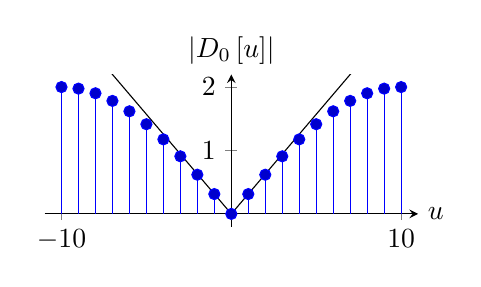
\begin{tikzpicture}
					\begin{axis} [width=180pt,height=100pt,
							axis x line=middle,
							axis y line=middle,
							tick align=center,
							every axis x label/.style={at={(current axis.right of origin)},anchor=west},
							every axis y label/.style={at={(current axis.above origin)}, anchor=north east,above=0mm},
							xmin=-11, xmax=11,
							xtick={-10, 0, 10},
							xlabel=$u$,
							ymin=-0.2, ymax=2.2,
							ytick={0,1,2},
							ylabel={$\left| D_0 \left[ u \right] \right|$}]
						\addplot+[ycomb,domain=-10:10,samples=21,samples y=0]
						({x}, {abs(2*sin(deg(pi*x/20)))});
						\addplot[domain=-10:10,samples=21,samples y=0]
						({x}, {abs(2*pi*x/20)});
					\end{axis}
				\end{tikzpicture}
				~ & ~
				\text{b)}
				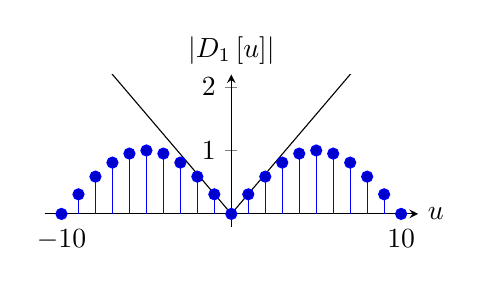
\begin{tikzpicture}
					\begin{axis} [width=180pt,height=100pt,
							axis x line=middle,
							axis y line=middle,
							tick align=center,
							every axis x label/.style={at={(current axis.right of origin)},anchor=west},
							every axis y label/.style={at={(current axis.above origin)}, anchor=north east,above=0mm},
							xmin=-11, xmax=11,
							xtick={-10, 0,10},
							xlabel=$u$,
							ymin=-0.2, ymax=2.2,
							ytick={0,1,2},
							ylabel={$\left| D_1 \left[ u \right] \right|$},
							color=black]
						\addplot+[ycomb,domain=-10:10,samples=21,samples y=0]
						({x}, {abs(sin(deg(2*pi*x/20)))});
						\addplot[domain=-10:10,samples=21,samples y=0]
						({x}, {abs(2*pi*x/20)});
					\end{axis}
				\end{tikzpicture}
			\end{array}
		\]
	\end{center}
	\caption{Magnitude of a) $D_0\left[u \right]$ and b) $D_1\left[u \right]$ and comparison with $\left| 2 \pi u/N \right|$, shown as a thin black line. Both DFT are computed over 20 samples.}
	\label{fig:d0andd1_dft}
\end{figure}

Derivates have become an important tool to represent images and they can be used to extract a great deal of information from the image as it was shown in the previous chapter. One thing about derivatives is that it might seem as we are loosing information from the input image. An important question is: if we have the derivative of a signal, can we recover the original image? what information is being lost? Intuitively, we should be able to recover the input image by integrating its derivative, but it is an interesting exercise to look in detail how this integration can be performed. We will start with a one dimensional signal and then we will discuss the two dimensional case.

A simple way of seeing that we can recover the input from its derivatives is to write the derivative in matrix form. This is the matrix that corresponds to the convolution with the kernel $\left[1, -1 \right]$ that we will call $D_0$. The next two matrices show the matrix $D_0$ and its inverse $D_0^{-1}$ for a 1D image of length 5 pixels using zero boundary conditions:
\begin{equation}
	D_0 =
	\begin{bmatrix}
		1 ~  & 0 ~  & 0 ~  & 0~   & 0 \\
		-1 ~ & 1 ~  & 0 ~  & 0~   & 0 \\
		0 ~  & -1 ~ & 1 ~  & 0 ~  & 0 \\
		0~   & 0 ~  & -1 ~ & 1 ~  & 0 \\
		0~   & 0 ~  & 0 ~  & -1 ~ & 1
	\end{bmatrix}
	~~~~~~~~~
	D^{-1} =
	\begin{bmatrix}
		1 ~ & ~ 0 ~ & ~ 0 ~ & ~ 0~  & ~ 0 \\
		1 ~ & ~ 1 ~ & ~ 0 ~ & ~ 0~  & ~ 0 \\
		1 ~ & ~ 1 ~ & ~ 1 ~ & ~ 0 ~ & ~ 0 \\
		1~  & ~ 1 ~ & ~ 1 ~ & ~ 1 ~ & ~ 0 \\
		1~  & ~ 1 ~ & ~ 1 ~ & ~ 1 ~ & ~ 1
	\end{bmatrix}
\end{equation}
We can see that the inverse $D^{-1}$ is reconstructing each pixel as a sum of all the derivate values from the left-most pixel to the right.  And the inverse perfectly reconstructs the input. But, this is cheating because the first sample of the derivative gets to see the actual value of the input signal and then we can integrate back the entire signal. That matrix is assuming zero boundary conditions for the signal and the boundary gives us the needed constraint to be able to integrate back the input signal.

But what happens if you only get to see differences and you remove any pixel that was affected by the boundary? In this case, the derivative operator in matrix form is:
\begin{equation}
	D_0 =
	\begin{bmatrix}
		-1 ~ & 1 ~  & 0 ~  & 0~   & 0 \\
		0 ~  & -1 ~ & 1 ~  & 0 ~  & 0 \\
		0~   & 0 ~  & -1 ~ & 1 ~  & 0 \\
		0~   & 0 ~  & 0 ~  & -1 ~ & 1
	\end{bmatrix}
\end{equation}

Let's consider the next 1D input signal:
\begin{equation}
	g = \left[1, 1, 2, 2, 0\right]
\end{equation}
then, the output of the derivative operator is:
\begin{equation}
	f=D_0g=\left[0, -1, 0, 2\right]
\end{equation}
Note that this vector has one sample less than the input.

To recover $g$ we can not invert $D_0$ as it is not a square matrix, but we can compute the pseudo inverse which turns out to be:
\begin{equation}
	D_0^{+} = \frac{1}{5}
	\begin{bmatrix}
		-4 ~ & -3 ~ & -2~  & -1 \\
		1 ~  & -3 ~ & -2 ~ & -1 \\
		1~   & 2 ~  & -2 ~ & -1 \\
		1~   & 2 ~  & 3 ~  & -1 \\
		1~   & 2 ~  & 3 ~  & 4
	\end{bmatrix}
\end{equation}
It has a funny structure and it is easy to see how it can be written in the general form for signals of length $N$. Also note that this is not a convolution.
Another important thing is that the inversion process is trying to recover more samples than there are observations. The trade off is that the signal that it will recover will have zero mean (so it looses one degree of freedom that can not be estimated). In this example, the reconstructed input is:
\begin{equation}
	\hat g = D^{+} f= \left[-0.2, -0.2, 0.8, 0.8, -1.2\right]
\end{equation}
Note that $\sum \hat g = 0$ and that this is $\hat g = g - 1.2$, where 1.2 is the mean value of samples on $g$.
Then, you still can recover the input signal up to the DC component.

In two dimensions things are a bit more complex. There are several ways in which partial image derivatives can be approximated. For instance, we can compute derivatives along the $n$ and $m$ components.

\begin{equation}
	\begin{bmatrix}
		1 \\
		-1
	\end{bmatrix}
	~
	\begin{bmatrix}
		1 -1
	\end{bmatrix}
\end{equation}

Or we can use a rotated reference frame as it is done in the Robert-Cross operator, introduced in 1963 \cite{} in a time when reading an image of $256 \times 256$ pixels into memory took several minutes:
% http://www.packet.cc/files/mach-per-3D-solids.html
\begin{equation}
	\begin{bmatrix}
		1 & ~0 \\
		0 & -1
	\end{bmatrix}
	~
	\begin{bmatrix}
		~0 & 1 \\
		-1 & 0
	\end{bmatrix}
\end{equation}

Although these operators are very old and better algorithms exist nowadays for edge extraction, when an efficient solution is needed, these simple operators are still very useful and had been used as key operators in modern computer vision descriptors such as HOG as we will see later.



Show some applications doing edge edition. This is a non-linear filter.



FIGURE: a) removing one object, b) moving one object from one image to another.

\subsection{Gaussian derivatives}

In the previous section we studied how to discretize derivatives. However, computing derivatives in practice has several difficulties. First, derivatives are sensitive to noise. In the presence of noise, as images tend to vary slowly, the difference between two continuous pixel values will be dominated by noise. There are also situations in which the derivative of an image is not defined. For instance, consider an image in the continuous domain with the form: $\img (x,y) = 0$ if $x<0$ and 1 otherwise. If we try to compute $\partial \img (x,y) / \partial x$ we will get 0 everywhere, but around $x=0$ the value of the derivative is not defined. We avoided this issue in the previous section as for discrete images the approximation of the derivative is always defined.

Gaussian derivatives address these two issues. They where introduced by Koendering and Van Doorm \cite{} as a model of the processing perform by neurons in the visual system.

Let's start with the following observation: For two functions defined in the continuous domain $f(x,y)$ and $g(x,y)$, we can write:
\begin{equation}
	\frac {\partial f(x,y)}{\partial x} \circ g(x,y) = f(x,y) \circ \frac {\partial g(x,y)}{\partial x}
\end{equation}
this is easy to prove in the Fourier domain. If our goal is to compute image derivatives and then blur the output using a low-pass filter, $g(x,y)$, then, instead of computing the derivative of the image we can compute the derivatives of the filter kernel and convolve it with the image. Even if the derivative of $f$ is not defined in some locations, we can always compute the result of this convolution.

If $g(x,y)$ is a blurring kernel it will smooth the derivatives reducing the output noise at the expense of a loss in spatial resolution. If $g$ is a Gaussian, then the derivative is:
\begin{equation}
	g_x(x,y; \sigma) = \frac {\partial g(x,y; \sigma)}{\partial x}= \frac{-x}{2 \pi \sigma^4} \exp{-\frac{x^2 +
			y^2}{2 \sigma^2}} = \frac{-x}{\sigma^2} g(x,y; \sigma)
	\label{eq:derivate1gauss2dcont}
\end{equation}
and the second order derivative is:
\begin{equation}
	g_{x^2}(x,y; \sigma) = \frac{x^2-\sigma^2}{\sigma^4} g(x,y; \sigma)
	\label{eq:derivate2gauss2dcont}
\end{equation}

\begin{figure}
	\begin{center}
		$
			\begin{array}{cc}
				\text{a)}
				\begin{tikzpicture}
					\begin{axis} [width=200pt,height=100pt,
							axis x line=middle,
							axis y line=middle,
							tick align=center,
							every axis x label/.style={at={(current axis.right of origin)},anchor=west},
							every axis y label/.style={at={(current axis.above origin)}, anchor=north east,above=0mm},
							xmin=-4, xmax=4,
							xtick={-3, -1, 0, 1, 3},
							xlabel=$x$,
							ymin=-0, ymax=.45,
							ytick={-.1,0.4},
							ylabel={$g(x)$}]
						\addplot[domain=-4:4,samples=101,samples y=0]
						({x}, {1/(sqrt(2*pi))*exp(-x*x/2)});
					\end{axis}
				\end{tikzpicture}
				~ & ~
				\text{b)}
				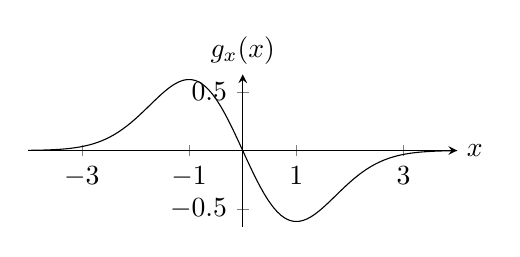
\begin{tikzpicture}
					\begin{axis} [width=200pt,height=100pt,
							axis x line=middle,
							axis y line=middle,
							tick align=center,
							every axis x label/.style={at={(current axis.right of origin)},anchor=west},
							every axis y label/.style={at={(current axis.above origin)}, anchor=north east,above=0mm},
							xmin=-4, xmax=4,
							xtick={-3, -1, 0, 1, 3},
							xlabel=$x$,
							ymin=-.65, ymax=.65,
							ytick={-0.5,0,0.5},
							ylabel={$g_x(x)$},
							color=black]
						\addplot[domain=-4:4,samples=101,samples y=0]
						({x}, {(-x)*exp(-x*x/2)});
					\end{axis}
				\end{tikzpicture}
				\\
				\text{c)}
				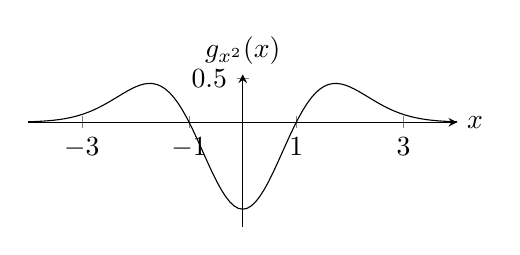
\begin{tikzpicture}
					\begin{axis} [width=200pt,height=100pt,
							axis x line=middle,
							axis y line=middle,
							tick align=center,
							every axis x label/.style={at={(current axis.right of origin)},anchor=west},
							every axis y label/.style={at={(current axis.above origin)}, anchor=north east,above=0mm},
							xmin=-4, xmax=4,
							xtick={-3, -1, 0, 1, 3},
							xlabel=$x$,
							ymin=-1.2, ymax=.55,
							ytick={0.5},
							ylabel={$g_{x^2}(x)$}]
						\addplot[domain=-4:4,samples=101,samples y=0]
						({x}, {(x*x-1)*exp(-x*x/2)});
					\end{axis}
				\end{tikzpicture}
				~ & ~
				\text{d)}
				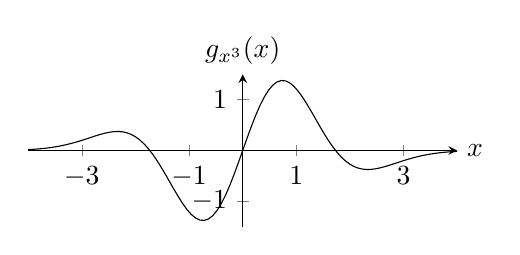
\begin{tikzpicture}
					\begin{axis} [width=200pt,height=100pt,
							axis x line=middle,
							axis y line=middle,
							tick align=center,
							every axis x label/.style={at={(current axis.right of origin)},anchor=west},
							every axis y label/.style={at={(current axis.above origin)}, anchor=north east,above=0mm},
							xmin=-4, xmax=4,
							xtick={-3, -1, 0, 1, 3},
							xlabel=$x$,
							ymin=-1.5, ymax=1.5,
							ytick={-1,0,1},
							ylabel={$g_{x^3}(x)$},
							color=black]
						\addplot[domain=-4:4,samples=101,samples y=0]
						({x}, {(-(x^3-3*x))*exp(-x*x/2)});
					\end{axis}
				\end{tikzpicture}
			\end{array}
		$
	\end{center}
	\caption{a) 1D Gaussian with $\sigma=1$ and b-d) its derivatives up to order 3.}
	\label{fig:d0andd1_dft}
\end{figure}

Each derivative can be written as the product between a polynomial on $x$, with the same order as the derivative, times a gaussian. The family of polynomials that result on computing gaussian derivatives is called Hermite polynomials. The general expression for the $n$ derivative of a gaussian is:
\begin{equation}
	g_{x^n}(x; \sigma) =
	\frac{\partial^{n} g(x)}{\partial x^n}
	=
	\left( \frac{-1}{\sigma \sqrt{2}} \right)^n
	H_n\left( \frac{x}{\sigma \sqrt {2}} \right)
	g(x; \sigma)
	\label{eq:derivate2gauss1dhermite}
\end{equation}
the first Hermite polynomial is $H_0(x)=1$, for $n=0$ we have the original Gaussian. Figure~\ref{fig:d0andd1_dft} shows the 1D Gaussian derivatives.

In two dimensions, as the gaussian is separable, the partial derivatives result on the product of two Hermite polynomial, one for each dimension:
\begin{equation}
	g_{x^n,y^m}(x,y; \sigma) =
	\frac{\partial^{n+m} g(x,y)}{\partial x^n \partial y^m}
	= %(-1)^{n+m}
	%\frac{1}{\sigma \sqrt{2}^{n+m}}
	\left( \frac{-1}{\sigma \sqrt{2}} \right)^{n+m}
	H_n\left( \frac{x}{\sigma \sqrt {2}} \right)
	H_m\left( \frac{y}{\sigma \sqrt {2}} \right)
	g(x,y; \sigma)
	\label{eq:derivate2gauss2dhermite}
\end{equation}
Figure~\ref{fig:gauss_derivatives_triangle} shows the 2D Gaussian derivatives, and Figure~\ref{fig:gauss_derivatives_triangle_FT} shows the corresponding Fourier transforms.


\begin{figure}
	\centerline{
		\includegraphics[width=0.8\linewidth]{figures/spatial_filters/gauss_derivatives_triangle.eps}}
	\caption{Gaussian derivatives up to order 6. All the kernels are separable. Although the seem similar to Fourier basis fig.~\ref{fig:gauss_derivatives_triangle_FT} shows that they are different to sine and cosine waves, instead they look more like products of cosine and sine waves.}
	\label{fig:gauss_derivatives_triangle}
\end{figure}


\begin{figure}
	\centerline{
		\includegraphics[width=0.8\linewidth]{figures/spatial_filters/gauss_derivatives_triangle_FT.eps}}
	\caption{Fourier transform of the Gaussian derivatives shown in figure~\ref{fig:gauss_derivatives_triangle}. Units are arbitrary.}
	\label{fig:gauss_derivatives_triangle_FT}
\end{figure}


The Gaussian derivatives share many of the properties of the Gaussian:
\begin{itemize}
	\item The convolution of two Gaussian derivatives of order $n$ and $m$ and variances $\sigma_1^2$ and $\sigma_2^2$ results in another gaussian derivative of order $n+m$ and variance $\sigma_1^2 + \sigma_2^2$. Proving this property on the spatial domain can be tedious. However it is trivial to prove it in the Fourier domain.
\end{itemize}



\begin{figure}
	$
		\begin{array}{ccc}
			\text{a)}
			\includegraphics[width=.3\linewidth]{figures/spatial_filters/gausian_der_c_2.jpg}
			 &
			\text{b)}
			\includegraphics[width=.3\linewidth]{figures/spatial_filters/gausian_der_c_4.jpg}
			 &
			\text{c)}
			\includegraphics[width=.3\linewidth]{figures/spatial_filters/gausian_der_c_8.jpg}
			\\
			\text{d)}
			\includegraphics[width=.3\linewidth]{figures/spatial_filters/gausian_der_c_2plot.jpg}
			 &
			\text{e)}
			\includegraphics[width=.3\linewidth]{figures/spatial_filters/gausian_der_c_4plot.jpg}
			 &
			\text{f)}
			\includegraphics[width=.3\linewidth]{figures/spatial_filters/gausian_der_c_8plot.jpg}
		\end{array}
	$
	\caption{An image filtered with three Gaussian derivatives with standard deviations: a) $\sigma=2$, b) $\sigma=4$, and c) $\sigma=8$. In the filtered images, bright pixels correspond to positive values and dark pixels correspond to negative values. Plots (d) - (f) show the three Gaussian derivatives over the same spatial support as the image. The discrete functions are approximated by sampling the continuous Gaussian derivatives. The convolutions are perform with mirror boundary conditions.}
	\label{fig:gaussiander_zebra}
\end{figure}


Figure~\ref{fig:gaussiander_zebra} shows an image filtered with three gaussian derivatives with different widths. Interestingly, derivatives at different scales emphasize different aspects of the image. The fine-scale derivatives (fig.~\ref{fig:gaussiander_zebra}.a) highlight the bands in the zebra, while the coarse-scale derivatives (fig.~\ref{fig:gaussiander_zebra}.c) emphasize more the object boundaries. This multiscale image analysis will be studied in depth in the following chapter.



When processing images we have to use discrete approximations for the Gaussian derivatives. After discretization, many of the properties of the continuous Gaussian will not hold exactly.

There are many discrete approximations. For instance, we can take samples of the continuous functions. In practice it is common to use the discrete approximation given by the binomial filters. Figure~\ref{fig:derivativepascaltriangle} shows the result of convolving the binomial coefficients with: $b_n \circ \left[1, -1\right]$.

\begin{figure}[h]
	\centerline{
		%\[
		$\begin{array}{ccccccccccccccccccccccccl}
				d_0 & ~ & ~ & ~ & ~ & ~ & ~    & ~    & ~    & ~    & ~    & ~~1  & ~~~ & -1  & ~  & ~  & ~  & ~  & ~  & ~ & ~ & ~ & ~ & ~ & \\
				d_1 & ~ & ~ & ~ & ~ & ~ & ~    & ~    & ~    & ~    & ~~1  & ~    & ~~0 & ~   & -1 & ~  & ~  & ~  & ~  & ~ & ~ & ~ & ~ & ~ & \\
				d_2 & ~ & ~ & ~ & ~ & ~ & ~    & ~    & ~    & ~~~1 & ~    & ~~~1 & ~~~ & -1  & ~  & -1 & ~  & ~  & ~  & ~ & ~ & ~ & ~ & ~ & \\
				d_3 & ~ & ~ & ~ & ~ & ~ & ~    & ~    & ~~~1 & ~    & ~~~2 & ~    & ~~0 & ~~~ & -2 & ~  & -1 & ~  & ~  & ~ & ~ & ~ & ~ & ~ & \\
				d_4 & ~ & ~ & ~ & ~ & ~ & ~    & ~~~1 & ~    & ~~~3 & ~    & ~~~2 & ~~~ & -2  & ~  & -3 & ~  & -1 & ~  & ~ & ~ & ~ & ~ & ~ & \\
				d_5 & ~ & ~ & ~ & ~ & ~ & ~~~1 & ~    & ~~~4 & ~    & ~~~5 & ~    & ~~0 & ~   & -5 & ~  & -4 & ~  & -1 & ~ & ~ & ~ & ~ & ~ &
			\end{array}$
		%\]
	}
	\caption{Derivative of binomial coefficients resulting from convolving $b_n \circ \left[1, -1\right]$. The first two filters are the ones we have studied in detail in the previous section.}
	\label{fig:derivativepascaltriangle}
\end{figure}

In two dimensions, we can use separable filters and build a partial derivative as:
\begin{equation}
	Sobel_x =  \begin{bmatrix}
		1 ~ & 0 ~ & -1 \\
	\end{bmatrix}\circ \begin{bmatrix}
		1 \\
		2 \\
		1
	\end{bmatrix}=
	\begin{bmatrix}
		1 ~ & 0 ~ & -1 \\
		2 ~ & 0 ~ & -2 \\
		1~  & 0 ~ & -1
	\end{bmatrix}
\end{equation}
\begin{equation}
	Sobel_y =  \begin{bmatrix}
		-1 & -2 & -1 \\
		~0 & ~0 & ~0 \\
		~1 & ~2 & ~1
	\end{bmatrix}
\end{equation}
This particular filter is called the Sobel-Feldman operator. The goal of this operator was to be compact and to be as isotropic as possible. The sobel-feldman operator can be implemented very efficiently as it can be written as the convolution with 4 small kernels: $Sobel_x=b_1 \circ d_0 \circ b_1^T \circ b_1^T$.  The DFT is:
\begin{equation}
	Sobel_x \left[u,v \right] = D_1\left[u\right] B_2 \left[v \right] = j \sin \left( 2 \pi u /N \right) \left( 2+2 \cos \left(2 \pi v/N \right) \right)
\end{equation}
and it is shown in fig.~\ref{fig:DFTderivativeoperators}.d. $N \times N$ is the extension of the domain (the operator is zero padded).

\begin{figure}
	\centerline{
		\includegraphics[width=1\linewidth]{figures/spatial_filters/DFTderivativeoperators.eps}}
	\caption{Magnitude of the DFT of four different discretization of Gaussian derivatives: a) $d_0$, b) $d_1$, c) Cross-Robert operator and d) Sobel-Feldman operator.  As $d_0$ and $d_1$ are one dimensional their 2D-DFT vary only along one dimension. The Cross-Robert operator is similar to a rotated version of $d_1$. The Sobel-Feldman operator has the profile of $D_1$ along the axis $u=0$ and it is proportional to the profile of $B_2$ along any section $v=constant$.
	}
	\label{fig:DFTderivativeoperators}
\end{figure}

Fig.~\ref{fig:DFTderivativeoperators} compares the DFT of the 4 types of approximations of the derivatives that we have discussed. These operators are still very popular. $Sobel$ has the best tolerance to noise due to its band-pass nature. The kernel $d_0$ is the one that provides the highest resolution in the output. Fig.~\ref{fig:circle} shows the output of different derivative approximations to a simple input image containing a circle. In the next section we will discuss now to use these derivatives to extract other interesting quantities.

% Sobel, I., Feldman, G., "A 3x3 Isotropic Gradient Operator for Image Processing", presented at the Stanford Artificial Intelligence Project (SAIL) in 1968. never published as a paper.
% https://www.researchgate.net/publication/239398674_An_Isotropic_3_3_Image_Gradient_Operator

\subsection{Image gradient and directional derivatives}

As we saw in chapter one, an important image representation is given by the image gradient. From the image derivatives we can define also the image gradient as the vector:
\begin{equation}
	\nabla \img = \left( \frac{\partial \img}{\partial x}, \frac{\partial \img}{\partial y} \right)
\end{equation}
For each pixel, the output is a two dimensional vector.  In the case of using gaussian derivatives, we can write:
\begin{equation}
	\nabla \img \circ g = \left( g_x(x,y), g_y(x,y) \right) \circ \img = \nabla g \circ \img
\end{equation}

Although we have mostly computed derivatives along the $x$ and $y$ variables, we can obtain the derivative on any orientation as a linear combination of the two derivatives along the main axes. With ${\bf t}=\left( \cos (\theta), \sin(\theta) \right)$, we can write the directional derivative a long the vector ${\bf t}$ as:
\begin{equation}
	\frac{\partial \img}{\partial {\bf t}} =  \nabla \img \cdot {\bf t} = \cos(\theta) \frac{\partial \img}{\partial x} + \sin(\theta) \frac{\partial \img}{\partial y}
\end{equation}
In the gaussian case:
\begin{equation}
	\frac{\partial \img}{\partial {\bf t}} \circ g = \left( \cos(\theta) g_x(x,y) + \sin(\theta) g_y(x,y) \right) \circ \img = \left( \nabla g  \cdot {\bf t} \right) \circ \img
	= g_{\theta} (x,y)  \circ \img
\end{equation}
with $g_{\theta} (x,y) = \cos(\theta) g_x(x,y) + \sin(\theta) g_y(x,y)$. However, to compute the derivate a long any arbitrary angle $\theta$ does not require doing new convolutions. Instead, we can compute any derivative as a linear combination of the output of convolving the image with $g_x(x,y)$ and $g_y(x,y)$:
\begin{equation}
	\frac{\partial \img}{\partial {\bf t}} \circ g =  \cos(\theta) g_x(x,y) \circ \img + \sin(\theta) g_y(x,y) \circ \img
\end{equation}

When using discrete convolutional kernels $d_n\left[n,m\right]$ and $d_m\left[n,m\right]$ to approximate the derivatives along $n$ and $m$, it can be written as:
\begin{equation}
	\nabla \img = \left( d_n\left[n,m\right], d_m\left[n,m\right] \right) \circ \img
\end{equation}
and
\begin{equation}
	\nabla \img \cdot {\bf t} =d_{\theta} \left[n,m\right] \circ \img
\end{equation}
with $d_{\theta} \left[n,m\right]  = \cos(\theta) d_n\left[n,m\right] + \sin(\theta) d_m\left[n,m\right]$. We expect that the linear combination of these two kernels should approximate the derivative in the direction $\theta$. The quality of this approximation will vary for the different kernels we have seen in the previous sections.


\begin{figure}
	\centerline{
		\includegraphics[width=1\linewidth]{figures/spatial_filters/circle.eps}}
	\caption{Image containing a circle filtered along the directions $n$, $m$ and 45 degrees. And also the magnitude and the angle of the gradient. The angle is shown only where the magnitude is $>0$. The derivative output along 45 degrees is obtained as a linear combination of the derivatives outputs along $n$ and $m$. Check the differences among the different kernels. The Sobel operator gives the most rotationally invariant gradient magnitude at the expense of a bit of blurring of the output.}
	\label{fig:circle}
\end{figure}



- The structure tensor: this is an example of a powerful image derivative representation. And we will see more of it (or related) later.

% - link to the work on scale space

\subsection{Laplacian}


\begin{figure}
	\begin{center}
		$
			\begin{array}{ccc}
				\text{a)}
				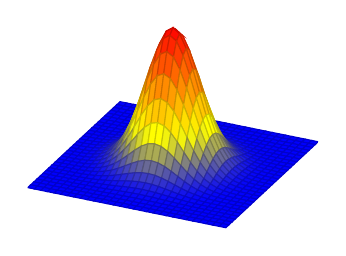
\begin{tikzpicture}
					\begin{axis}
						[width=150pt,height=150pt,
							xmin=-4, xmax=4,
							%xtick={-3, -1, 0, 1, 3},
							xlabel=$x$,
							ymin=-4, ymax=4,
							%ytick={-1,0,1},
							ylabel={$y$},
							hide axis,
							colormap/hot]
						\addplot3[domain=-4:4,samples=31,
							surf,
						]
						{1/(2*pi)*exp(-(x^2+y^2)/2)};
					\end{axis}
				\end{tikzpicture}
				 &
				\text{b)}
				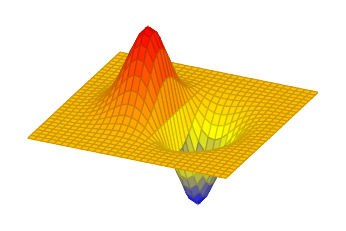
\begin{tikzpicture}
					\begin{axis}
						[width=150pt,height=150pt,
							xmin=-4, xmax=4,
							%xtick={-3, -1, 0, 1, 3},
							xlabel=$x$,
							ymin=-4, ymax=4,
							%ytick={-1,0,1},
							ylabel={$y$},
							hide axis,
							axis lines = left,
							colormap/hot]
						\addplot3[domain=-4:4,samples=31,
							surf,
						]
						{1/(2*pi)*(-x)*exp(-(x^2+y^2)/2)};
					\end{axis}
				\end{tikzpicture}
				 &
				\text{c)}
				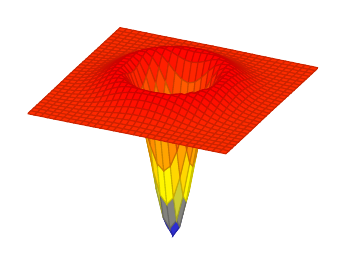
\begin{tikzpicture}
					\begin{axis}
						[width=150pt,height=150pt,
							xmin=-4, xmax=4,
							%xtick={-3, -1, 0, 1, 3},
							xlabel=$x$,
							ymin=-4, ymax=4,
							%ytick={-1,0,1},
							ylabel={$y$},
							hide axis,
							axis lines = left,
							colormap/hot]
						\addplot3[domain=-4:4,samples=31,
							surf,
						]
						{1/(2*pi)*(x^2+y^2-2)*exp(-(x^2+y^2)/2)};
					\end{axis}
				\end{tikzpicture}
			\end{array}
		$
	\end{center}
	\caption{Three 2D gaussian-related convolutional kernels: a) 2D gaussian with $\sigma=1$, b) its $x$ derivative, and c) its laplacian.}
	\label{fig:threekernels}
\end{figure}

The Laplacian filter was made popular by Marr and Hildreth in 1980 \cite{} in the search for operators that locate the boundaries between objects. The Laplacian is a common operator from differential geometry to measure the divergence of the gradient and it appears frequently in modeling fields in physics. One cool example is the paper "can one hear the shape of a drum" \cite{} where the laplacian is used for modeling vibrations in a drum and the sounds it produces as a function of its shape, those results have applications also in spectral methods for image segmentation as we will see later.
%Can one hear the shape of a drum. The American Mathematical Monthly, vol. 73, 1966, Part II, pp. 1-23

The Laplacian operator is defined as the sum of the second order partial derivatives of a function:
% Marr, D.; Hildreth, E. (29 Feb 1980), "Theory of Edge Detection", Proceedings of the Royal Society of London. Series B, Biological Sciences 207 (1167): 187�217
\begin{equation}
	\nabla^2 \img = \frac{\partial^2 \img}{\partial x^2} + \frac{\partial^2 \img}{\partial y^2}
\end{equation}
The laplacian is more sensitive to noise than the first order derivatives. Therefore, in the presence of noise, it is useful to filter the output with a gaussian. We can write:
\begin{equation}
	\nabla^2 \img \circ g = \nabla^2 g \circ \img
\end{equation}
Where
\begin{equation}
	\nabla^2 g = \frac{x^2 + y^2 -2\sigma^2}{\sigma^4} g(x,y)
\end{equation}

Figure \ref{fig:threekernels} compares the 2D gaussian laplacian (fig.~\ref{fig:threekernels}.c) with the first order derivative (fig.~\ref{fig:threekernels}.b) of a 2D gaussian (fig.~\ref{fig:threekernels}.a). Due to its shape, the laplacian is also called the inverted mexican hat wavelet. Despite that visually it might seem as if the laplacian has a negative mean the mean is actually zero as the positive side is wider than the negative. Figure \ref{fig:DFTlaplacians} shows the DFT of the gaussian laplacian for three different values of $\sigma$. For values $\sigma>1$ the resulting filter is band-pass.

\begin{figure}
	\centerline{
		\includegraphics[width=1\linewidth]{figures/spatial_filters/DFTlaplacians.eps}}
	\caption{Magnitude of the DFT of the Gaussian Laplacian with three different widths and a discrete approximation: a) $\sigma=1/2$, b) $\sigma=1$, c) $\sigma=2$ and d) DFT of the five-point discrete approximation to the laplacian.
	}
	\label{fig:DFTlaplacians}
\end{figure}

In the discrete domain there are several approximations to the laplacian filter. Lindeberg \cite{} explored different approximations to the image Laplacian in order to optimize its properties. In one dimension, the Laplacian can be approximated by $\left[ 1,-2,1 \right]$ which is the result of the convolution of $\left[1,-1 \right] \circ \left[1,-1 \right]$.
% ftp://ftp.nada.kth.se/CVAP/reports/cvap66.pdf
In two dimensions, the most popular approximation is the five-point formula which consists in convolving the image with the kernel:
\begin{equation}
	\nabla_5^2 =
	\begin{bmatrix}
		0 & 1  & 0 \\
		1 & -4 & 1 \\
		0 & 1  & 0
	\end{bmatrix}
\end{equation}
It involves the central pixel and its four nearest neighbors. This is a sum-separable kernel: it corresponds to approximating the second order derivative for each coordinate and summing the result (i.e., convolve the image with $\left[1,-2,1\right]$ and also with its transpose and summing the two outputs. It is important to shift by one pixel, on the appropriate dimension, the two results to make sure that the sum results in the Laplacian.) Figure \ref{fig:threekernels}.d shows the DFT of this approximation. It also has a quadratic from near the origin of the frequency domain, but it has a high-pass shape similar to the one obtained for a small value of $\sigma$.

Note that when summing two first order derivatives along $x$ and $y$, what we obtain is a first order derivative along the 45 degrees angle. However, when summing up the two second order derivatives we obtain a rotationally invariant kernel. This is shown in fig.~\ref{fig:wheellaplacian}


\begin{figure}
	$
		\begin{array}{cccc}
			\text{a)}
			\includegraphics[width=.222\linewidth]{figures/spatial_filters/wheel256.jpg}
			 &
			\text{b)}
			\includegraphics[width=.222\linewidth]{figures/spatial_filters/wheelLaplacianx.jpg}
			 &
			\text{c)}
			\includegraphics[width=.222\linewidth]{figures/spatial_filters/wheelLaplaciany.jpg}
			 &
			\text{d)}
			\includegraphics[width=.222\linewidth]{figures/spatial_filters/wheelLaplacian.jpg}
		\end{array}
	$
	\caption{a) Input image, b) second order derivative along $x$, c) second order derivative along $y$ and d) the sum of the two second order derivatives, which results in the laplacian output.}
	\label{fig:wheellaplacian}
\end{figure}



%FIGURE: a) continuous laplacian of a gaussian, b) FT of the gaussian laplacian. c) DFT of the discrete 5-point approximation.

The discrete approximation also provides a better intuition of how it works than its continuous counterpart. The Laplacian filter has a number of advantages with respect to the gradient:
\begin{itemize}
	\item It is rotationally invariant: it is a linear operator that responds equally to edges in any orientation (this is only approximate in the discrete case).
	\item It measures curvature: if the image contains a linear trend the derivative will be non-zero despite being no boundaries, while the laplacian will be zero.
	\item Edges can be located as the zero-crossings in the Laplacian output. However, this way of detecting edges is not very reliable.
	\item Zero crossings of an image form closed contours.
\end{itemize}

Marr-Hildreth \cite{} used zero-crossings of the laplacian output to compute edges, but this method is not used nowadays for edge detection. Instead the laplacian filter is widely used in a number of other image representations. It is used to build image pyramids (multiscale representations, chapter~\ref{}), to detect points of interest in images (it is the basic operator used to detect keypoints where to compute SIFT descriptors, which we will discuss in chapter~\ref{}).

Figure~\ref{fig:discretelaplacian1d} compares the output of the first order derivative (Fig.~\ref{fig:discretelaplacian1d}.b) and the laplacian (Fig.~\ref{fig:discretelaplacian1d}.d) on a simple 1D signal (Fig.~\ref{fig:discretelaplacian1d}.a). The local maximum of the derivative output (Fig.~\ref{fig:discretelaplacian1d}.c) and the zero crossings of the laplacian output (Fig.~\ref{fig:discretelaplacian1d}.e) are aligned with the transitions (boundaries) of the input signal (Fig.~\ref{fig:discretelaplacian1d}.a).

\begin{figure}[h]
	\begin{center}
		$
			\begin{array}{lcr}
				~ & ~ &
				\text{a)}
				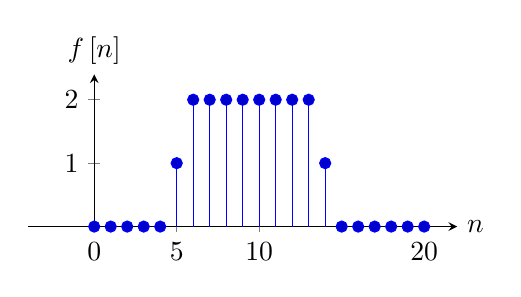
\begin{tikzpicture}
					\begin{axis} [width=200pt,height=100pt,
							axis x line=bottom,
							axis y line=middle,
							tick align=center,
							every axis x label/.style={at={(current axis.right of origin)},anchor=west},
							every axis y label/.style={at={(current axis.above origin)}, anchor=north east,above=0mm},
							xmin=-4, xmax=22,
							xtick={0, 5,10, 20},
							xlabel=$n$,
							ymin=0, ymax=2.4,
							ytick={0,...,2},
							ylabel={$f \left[n\right]$}]
						\addplot+[ycomb] plot coordinates {(0,0) (1,0) (2,0) (3,0) (4,0) (5,1) (6,2) (7,2) (8,2) (9,2) (10,2) (11,2) (12,2) (13,2) (14,1) (15,0) (16,0) (17,0) (18,0) (19,0) (20,0)};
					\end{axis}
				\end{tikzpicture}
				\\
				\text{b)}
				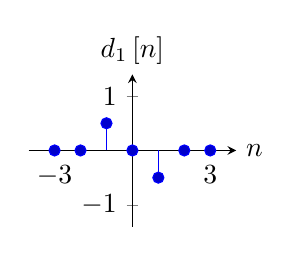
\begin{tikzpicture}
					\begin{axis} [width=120pt,height=100pt,
							axis x line=middle,
							axis y line=middle,
							tick align=center,
							every axis x label/.style={at={(current axis.right of origin)},anchor=west},
							every axis y label/.style={at={(current axis.above origin)}, anchor=north east,above=0mm},
							xmin=-4, xmax=4,
							xtick={-3,3},
							xlabel=$n$,
							ymin=-1.4, ymax=1.4,
							ytick={-1,0,1},
							ylabel={$d_1 \left[n\right]$},
							color=black]
						\addplot+[ycomb] plot coordinates {(-3,0) (-2,0) (-1,1/2) (0,0) (1,-1/2) (2,0) (3,0) };
					\end{axis}
				\end{tikzpicture}
				  &
				~
				  &
				\text{c)}
				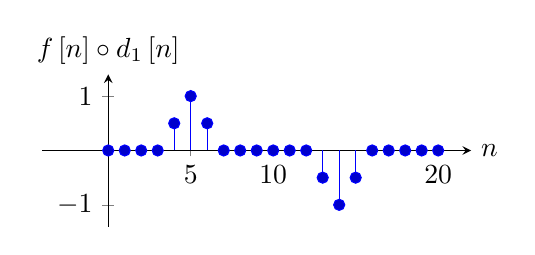
\begin{tikzpicture}
					\begin{axis} [width=200pt,height=100pt,
							axis x line=middle,
							axis y line=middle,
							tick align=center,
							every axis x label/.style={at={(current axis.right of origin)},anchor=west},
							every axis y label/.style={at={(current axis.above origin)}, anchor=north east,above=0mm},
							xmin=-4, xmax=22,
							xtick={0, 5,10, 20},
							xlabel=$n$,
							ymin=-1.4, ymax=1.4,
							ytick={-1,...,1},
							ylabel={$f \left[n\right] \circ d_1 \left[n\right]$}]
						%\addplot+[ycomb] plot coordinates {(0,0) (1,0) (2,0) (3,0) (4,0) (5,1) (6,2) (7,2) (8,2) (9,2) (10,2) (11,2) (12,2) (13,2) (14,1) (15,0) (16,0) (17,0) (18,0) (19,0) (20,0)};
						\addplot+[ycomb] plot coordinates {(0,0) (1,0) (2,0) (3,0) (4,1/2) (5,1) (6,1/2) (7,0) (8,0) (9,0) (10,0) (11,0) (12,0) (13,-1/2) (14,-1) (15,-1/2) (16,0) (17,0) (18,0) (19,0) (20,0)};
					\end{axis}
				\end{tikzpicture}
				\\
				\text{d)}
				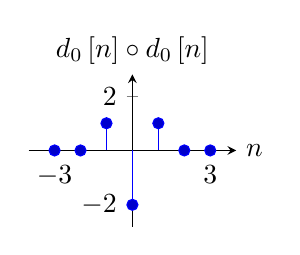
\begin{tikzpicture}
					\begin{axis} [width=120pt,height=100pt,
							axis x line=middle,
							axis y line=middle,
							tick align=center,
							every axis x label/.style={at={(current axis.right of origin)},anchor=west},
							every axis y label/.style={at={(current axis.above origin)}, anchor=north east,above=0mm},
							xmin=-4, xmax=4,
							xtick={-3,3},
							xlabel=$n$,
							ymin=-2.8, ymax=2.8,
							ytick={-2,0,2},
							ylabel={$d_0 \left[n\right] \circ d_0 \left[n\right]$},
							color=black]
						\addplot+[ycomb] plot coordinates {(-3,0) (-2,0) (-1,1) (0,-2) (1,1) (2,0) (3,0) };
					\end{axis}
				\end{tikzpicture}
				  &
				~
				  &
				\text{e)}
				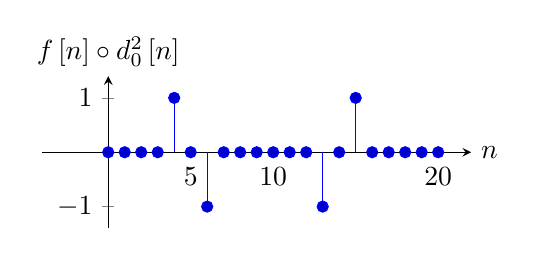
\begin{tikzpicture}
					\begin{axis} [width=200pt,height=100pt,
							axis x line=middle,
							axis y line=middle,
							tick align=center,
							every axis x label/.style={at={(current axis.right of origin)},anchor=west},
							every axis y label/.style={at={(current axis.above origin)}, anchor=north east,above=0mm},
							xmin=-4, xmax=22,
							xtick={0, 5,10, 20},
							xlabel=$n$,
							ymin=-1.4, ymax=1.4,
							ytick={-1,...,1},
							ylabel={$f \left[n\right] \circ d_0^2 \left[n\right]$}]
						%\addplot+[ycomb] plot coordinates {(0,0) (1,0) (2,0) (3,0) (4,0) (5,1) (6,2) (7,2) (8,2) (9,2) (10,2) (11,2) (12,2) (13,2) (14,1) (15,0) (16,0) (17,0) (18,0) (19,0) (20,0)};
						\addplot+[ycomb] plot coordinates    {(0,0) (1,0) (2,0) (3,0) (4,1) (5,0) (6,-1) (7,0) (8,0) (9,0) (10,0) (11,0) (12,0) (13,-1) (14,0) (15,1) (16,0) (17,0) (18,0) (19,0) (20,0)};
					\end{axis}
				\end{tikzpicture}
			\end{array}
		$
	\end{center}
	\caption{Comparison between the output of a first order derivative and the Laplacian of 1D signal. a) Input signal, b) kernel $d_1$, c) output of the derivative (convolution of (a) and (b)), d) discrete approximation of the Laplacian and e) output of convolving the signal (a) with the laplacian kernel (d).}
	\label{fig:discretelaplacian1d}
\end{figure}


The Laplacian filter can also be used as a coarse approximation of the behavior of the early visual system. When looking at the magnitude of the DFT of the laplacian with $\sigma=1$ (fig.~\ref{fig:DFTlaplacians}), the shape seems reminiscent of our subjective evaluation of our own visual sensitivity to spatial frequencies when we look at the Campbell \& Robson chart (fig.~\ref{fig:csfchart}). As the visual filter does not seem to cancel exactly the very low spatial frequencies as the laplacian does, a better approximation is:
\begin{equation}
	h = \nabla^2 g  + \lambda g
	\label{eq:humanmodel}
\end{equation}
where $h$ is the approximate impulse response of the human visual system, $\lambda$ is a small constant that is equal to the DC gain of the filter. This particular form of the human sensitivity function helps to explain some visual illusions. One of them is shown in figure \ref{fig:vasarely}. This visual illusion is called the Vasarely visual illusion. Images (a) and (d) show two gray-scale pyramids  formed by superimposing squares of increasing (or decreasing) intensity. When looking at them we perceive the diagonal directions as being brighter (a) or darker (d) than their neighborhood. This is an illusion because there is not such a difference in image intensity.  One explanation consists in saying that the image that we perceive is the output of a filter (as shown in eq.~\ref{eq:humanmodel}). Images (b) and (e) show the output of such a filter. We can see the diagonals again as being brighter or darker but now this effect is not an illusion, the brighter and darker diagonals are really part of the filtered image. In fact, (c) shows in blue an horizontal section at one quarter of image (b). The red curve is the section of the input image (a). We can see that the output really contains a pick in intensity on the diagonals of image (b). The plot in figure (f) shows the same for images (d) and (e).

\begin{figure}
	$
		\begin{array}{ccc}
			\text{a)}
			\includegraphics[width=.3\linewidth]{figures/spatial_filters/vasarely_c.jpg}
			 &
			\text{b)}
			\includegraphics[width=.3\linewidth]{figures/spatial_filters/vasarely_d.jpg}
			 &
			\text{c)}
			\includegraphics[width=.3\linewidth]{figures/spatial_filters/vasarely_section.eps}
			\\
			\text{d)}
			\includegraphics[width=.3\linewidth]{figures/spatial_filters/vasarely_a.jpg}
			 &
			\text{e)}
			\includegraphics[width=.3\linewidth]{figures/spatial_filters/vasarely_b.jpg}
			 &
			\text{f)}
			\includegraphics[width=.3\linewidth]{figures/spatial_filters/vasarely_section_b.eps}
		\end{array}
	$
	\caption{Vasarely visual illusion. Images (a) and (d) show two gray-scale pyramids. When looking at them we perceive the diagonal directions as being brighter (a) or darker (d) than their neighborhood. Images (b) and (e) show the output of the human model given by the filter from eq.~\ref{eq:humanmodel}. The plots (c) and (f) show, in blue, an horizontal section at one quarter of image (b) and (e) showing the intensity profile as a function of $x$. The red curve is the section of the corresponding input image. We can see that the output really contains a pick in intensity on the diagonals of the input image.}
	\label{fig:vasarely}
\end{figure}



%FIGURE: Show Vasarely illusion (http://web.mit.edu/persci/people/adelson/publications/gazzan.dir/vasarely.html)

% https://en.wikipedia.org/wiki/Discrete_Laplace_operator


\section{Applications}


\subsection{Sharpening filter}

One example of a simple but very useful filter is a sharpening filter. The goal of a sharpening filter is to transform an image so that it appears sharper. This can be achieved by amplifying the amplitude of the high-spatial frequency content of the image. We can achieve this with a combination of filters that we have already discussed in this section.

%\begin{figure}
%\centerline{
%\includegraphics[width=1\linewidth]{figures/intro_signals/sharpened.jpg}}
%\caption{ Sharpening achieved by subtraction of blurred
%  components (the three filter taps of amplitude $\frac{1}{3}$) from
%  the full image (scaled appropriately). 
%} 
%\label{fig:convExamps3}
%\end{figure}

\begin{figure}
	$
		\begin{array}{ccc}
			\text{a)}
			\includegraphics[width=.3\linewidth]{figures/spatial_filters/boat_sharp.jpg}
			 &
			\text{b)}
			\includegraphics[width=.3\linewidth]{figures/spatial_filters/boat_sharp0.jpg}
			 &
			\text{c)}
			\includegraphics[width=.3\linewidth]{figures/spatial_filters/boat_sharp1.jpg}
			\\
			\text{d)}
			\includegraphics[width=.3\linewidth]{figures/spatial_filters/boat_sharp2.jpg}
			 &
			\text{e)}
			\includegraphics[width=.3\linewidth]{figures/spatial_filters/boat_sharp3.jpg}
			 &
			\text{f)}
			\includegraphics[width=.3\linewidth]{figures/spatial_filters/boat_sharp4.jpg}
		\end{array}
	$
	\caption{Sharpening achieved by subtraction of blurred components. a) Original image, b) sharpened once by filtering with kernel from eq.~\ref{eq:sharpening}.  Each color channel is filtered independently. c) - f) the same filter is applied successively to the previous output. In the last image the sharpening filter has been applied 5 times to the input image. The last image seems looks substantially sharper than the original image, but close inspection will reveal some artifacts.}
	\label{fig:convExamps3}
\end{figure}



A simple way to design a {\em sharpening} filter is
to de-emphasize the blurry components of an image.  By the linearity
of the convolution operator, we're allowed to add and
subtract kernels to make a new kernel that would give us the same
filtered image as if we had added and subtracted the filtered outputs
of each of the component kernels.  For this example, we start with
twice the original image (sharp plus blurred parts), then subtract
away  the blurred components of the image:
\begin{equation}
	\text{sharpening filter} =
	\begin{bmatrix}
		0 & 0 & 0 \\
		0 & 2 & 0 \\
		0 & 0 & 0
	\end{bmatrix}
	-
	\frac{1}{16}
	\begin{bmatrix}
		1 & 2 & 1 \\
		2 & 4 & 2 \\
		1 & 2 & 1
	\end{bmatrix}
	\label{eq:sharpening}
\end{equation}
Note that the DC gain of this sharpening filter is 1. That would leave
one original image in there, plus an additional component of the sharp
details.  The perceptual result is that of a sharpened image, Fig.~\ref{fig:convExamps3}. We can apply this filter successively in order to further enhance the image details. If too much sharpening is applied we might end up enhancing noise and introducing image artifacts.



%\subsection{Motion blur and camera shake.}

%The Gaussian filter that we have studied can be used to model how images are blur when a picture is taken out of focus, or when we remove the eyeglasses. But there are other types of image blur that also happen in natural situations.  Figure~\ref{fig:motions} shows examples of linear motion blur (fig~\ref{fig:motions}.a-c), and camera shake  (fig~\ref{fig:motions}.d-i). Motion blur happens when there are objects moving in the scene or when the camera is moving while the shutter is open. 
%Camera shake is produced due to the small camera vibration that happens while taking a picture and it is more important under low-light conditions. Camera shake can be modeled as a blur kernel, describing the camera motion during exposure, convolved with the image intensities. Depending on the shake the resulting picture looks as 


%\begin{figure}
%$
%\begin{array}{ccc}
%\text{a)}
%\includegraphics[width=.38\linewidth]{figures/intro_signals/street.jpg}
%&
%\text{b)}
%\includegraphics[width=.15\linewidth]{figures/intro_signals/blur_kernel2.jpg}
%&
%\text{c)}
%\includegraphics[width=.38\linewidth]{figures/intro_signals/street_kernel2.jpg}
%\\
%\text{d)}
%\includegraphics[width=.38\linewidth]{figures/intro_signals/bostonnight.jpg}
%&
%\text{e)}
%\includegraphics[width=.15\linewidth]{figures/intro_signals/blur_kernel5.jpg}
%&
%\text{f)}
%\includegraphics[width=.38\linewidth]{figures/intro_signals/bostonnight_kernel5.jpg}
%\\
%\text{g)}
%\includegraphics[width=.38\linewidth]{figures/intro_signals/stata.jpg}
%&
%\text{h)}
%\includegraphics[width=.15\linewidth]{figures/intro_signals/stata_blur.jpg}
%&
%\text{i)}
%\includegraphics[width=.38\linewidth]{figures/intro_signals/stata_blurry.jpg}
%\end{array}
%$
%\caption{a) Simulated motion blur, in this case it is produced because the picture is taken from a moving car. d) Simulated camera shake blur (the camera has followed a circular trajectory while the shutter was open). Probably the reader has seen this type of effect in some pictures taken at night.} 
%\label{fig:motions}
%\end{figure}

%Figure~\ref{fig:motions}.d-i shows one simulated example of camera shake. In this case, the photographer is trying to capture the scene shown in fig.~\ref{fig:motions}.d, but during exposure the camera followed a circular path. Therefore, the resulting picture (fig.~\ref{fig:motions}.f) is the convolution of the ideal picture (fig.~\ref{fig:motions}.d) with the convolution kernel (fig.~\ref{fig:motions}.e). The result has probably a familiar effect for anyone that has taken pictures at night. The light sources in the picture are like delta functions that produce multiple copies of the convolution kernel. Figure~\ref{fig:motions}.g-i shows a different example where the camera has follow a more complex trajectory.

%It will be nice to have tools capable to removing the effect of camera motion to produce sharp pictures. This is an active area of research and we will discuss approaches to this problem in chapter \ref{}.


% These are blurs that happen in nature but that are complicated even for the eye. They are convolutions but sometimes we can not write analytic functions for describing them. But they are very important. The eye can tell them apart (make a figure with the same image filtered with different blur filters) but it might have difficulties in seeing in the presence of these blurs. This is why reversing the effect of these blurs is very important and very difficult.

%Make some examples: 

% $h\left[n,m\right] = \delta \left[n-1,m\right] +  \delta \left[n+5,m-3\right]$. This filter makes the image to appear twice. This happens sometimes when taking pictures. It is not nice when a picture turns out like that and it will be nice to have tools to remove it, but reversing it is hard... Can we compute the inverse? Can we filter back the signal? We will see how to do this in a later chapter.


\subsection{Artistic filters}

Despite the simplicity of linear filters, they can be used to produce pleasing artistic effects. Combining linear filters with some simple non-linearities provides a very large number of possibilities. These types of image manipulation techniques are very popular as they can be implemented very efficiently and can be computed very fast even on mobile devices. Linear convolutional filters are the basis of applications such as Photoshop or Instagram.

Exploring artistic effects and playing with filters to enhance pictures is a nice way of learning and gaining intuition about linear filter theory. Figure~\ref{fig:arteffects} shows a few linear filters and the result they have in images. Those filters are easy to implement and will allow you creating nice effects.

\begin{figure}
	$
		\begin{array}{ccc}
			\text{a)}
			\includegraphics[width=.38\linewidth]{figures/spatial_filters/boat.jpg}
			 &
			\text{b)}
			\includegraphics[width=.15\linewidth]{figures/spatial_filters/boat_kernel.jpg}
			 &
			\text{c)}
			\includegraphics[width=.38\linewidth]{figures/spatial_filters/boat_effect.jpg}
			\\
			\text{d)}
			\includegraphics[width=.38\linewidth]{figures/spatial_filters/trees.jpg}
			 &
			\text{e)}
			\includegraphics[width=.15\linewidth]{figures/spatial_filters/kernel2transpose.jpg}
			 &
			\text{f)}
			\includegraphics[width=.38\linewidth]{figures/spatial_filters/trees_kernel2.jpg}
		\end{array}
	$
	\caption{Simple linear filters can create interesting effects. a-c) Random kernel. Here, by filtering the image (a) with a random set of impulses (b) at random locations and random positive amplitudes, creates an image that seems to be drawn with a pencil (c). In this example, the image is $512 \times 512$ pixels and the kernel has a support of $64 \times 64$ pixels with 50 random dots with random amplitudes between 0.5 and 1. Each color channel is filtered independently with the same kernel. d-f) Vertical motion blur.}
	\label{fig:arteffects}
\end{figure}


Intentional motion blur that can be achieved by moving the camera  while taking a picture. The example in figure~\ref{fig:arteffects}.f simulates the effect of moving the camera up and down. The linear filtering produces an interesting effect on the tree trunks making them become more visually salient while attenuating other image details.

% https://ebgriffith.wordpress.com/tag/effect/

%\subsection{Bio-inspired filters}


%End-stopping

%Hubel and Viesel


\section{Concluding remarks}

%In this chapter we have talked about:
%\begin{itemize}
%\item Signals, images
%\item Representations in the Space and frequency domain
%\end{itemize}

Important topics that we have not described:
\begin{itemize}
	\item We have not gone in detail in recursive filters. Maybe we should add another example in the temporal domain?
	\item We have not described how to connect difference equations and the transfer function of a system.
	\item We have not described how to analyze the stability of recursive systems.
	\item Feedback and feedforward systems
\end{itemize}

% Note from antonio: Neuromorphic circuits make sense here as a first application of all the tools they have seen already. They do not need to understand quadrature or pyramids in order to understand this section.

%\input{neuro}

